\section{Metodologia dos experimentos}
\label{sec:dtw-metodology}

A metodologia utilizada neste modelo pode ser dividido em duas partes: (1) como os dados do banco de dados foram organizados e; (2) como funciona o processo de identificação das janelas do banco de dados.

\subsection{Organização do banco de dados de referência}

Como mencionado na \subsecref{subsec:indexation_and_identification}, o banco de dados de referência para esse modelo respeita um conjunto de três regras. Portanto, para os nossos experimentos, precisamos organizar as sequências de referência de acordo.

Uma forma de visualizar como os dados podem ser estruturados é transformando as sessões de uma música em uma espécie de máquina de estados, como a ilustrada na \figref{fig:miab_state_machine} da música \textit{Message In A Bottle} para a trilha da guitarra elétrica de base. Como exemplo, em um corte da partitura da música, demonstrada na \figref{fig:miab_sheet_music}, é possível visualizar como esses estados estão organizados. 

\begin{figure}[htbp]
    \centering
    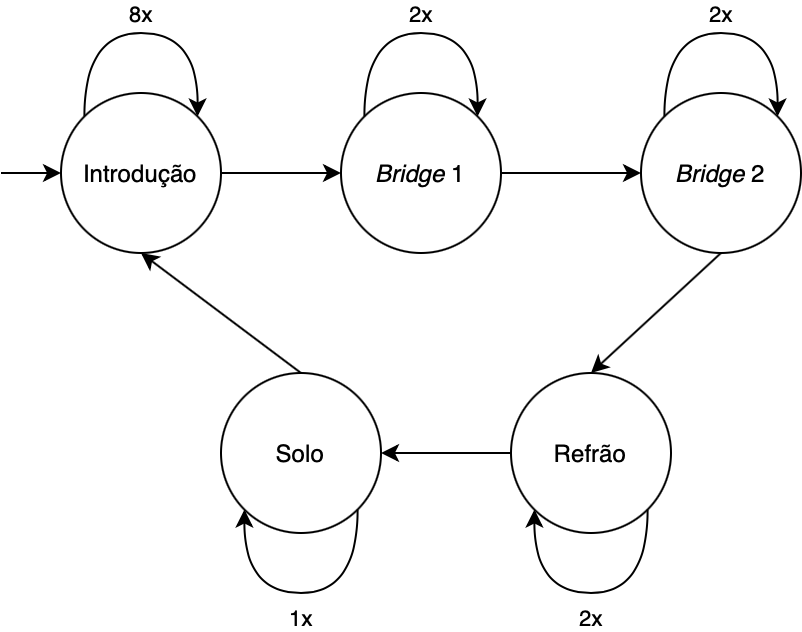
\includegraphics[width=0.75\textwidth]{images/MIAB state machine.png}
    \caption{Máquina de estados para a trilha da guitarra elétrica de base da música \textit{Message In A Bottle} (\textit{The Police}, 1979).}
    \label{fig:miab_state_machine}
\end{figure}

\begin{figure}[htbp]
    \centering
    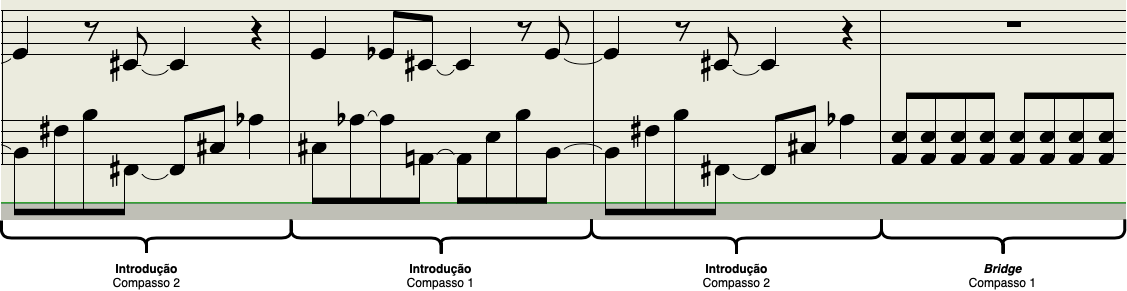
\includegraphics[width=1\textwidth]{images/dtw-real division.png}
    \caption{Relação dos estados da \figref{fig:miab_state_machine} com compassos na partitura da trilha da guitarra elétrica da música \textit{Message In A Bottle} (\textit{The Police}, 1979).}
    \label{fig:miab_sheet_music}
\end{figure}

No entanto, é notável que alguns estados podem transitar para mais de um estado. Por exemplo, a introdução pode transitar entre si mesma em um \textit{loop} ou para o \textit{bridge}. Tal característica quebra a Regra 3, pois, caso o estado identificado fosse a introdução, não seria possível saber qual seria o próximo estado e duas previsões seriam entregues, causando ambiguidade.

Para lidar com isso, podemos reorganizar tal máquina apresentando estados de transição. Dessa forma, quando uma transição fosse identificada, apenas uma previsão seria gerada, como ilustrado na \figref{fig:miab_adapted_state_machine}. Note, entretanto, que nenhum dos estados ``aponta'' para um estado de transição. Isso significa os cortes de áudio que representam essas transições nunca será apontado como uma previsão, efetivamente perdendo essa informação na transmissão do músico remoto.

\begin{figure}[htbp]
    \centering
    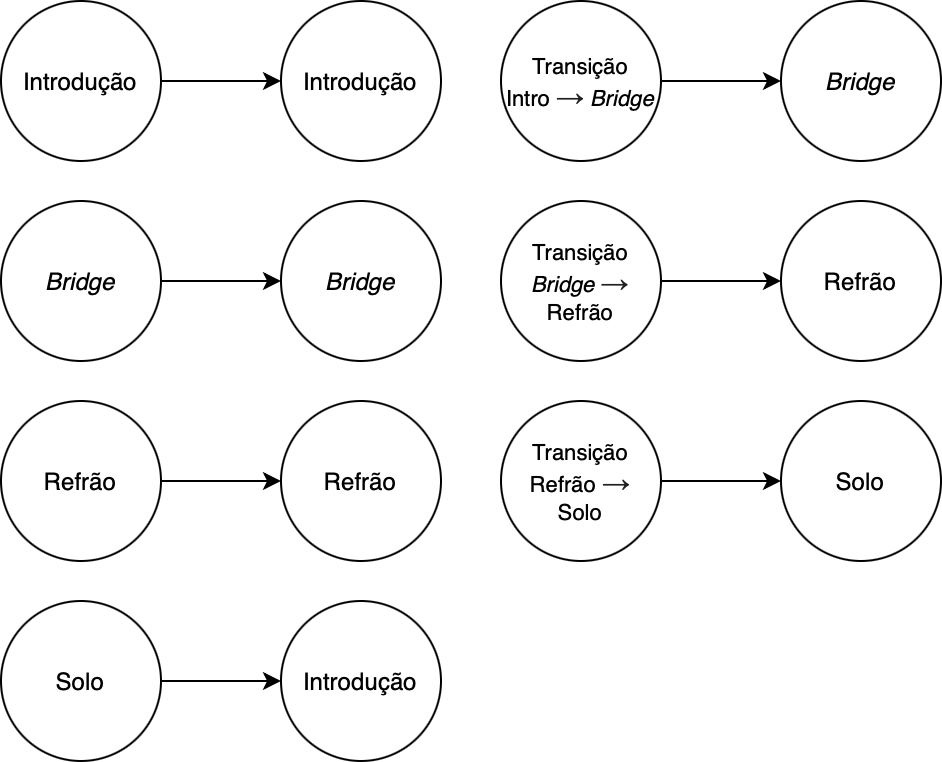
\includegraphics[width=0.75\textwidth]{images/MIAB adapted state machine.png}
    \caption{Máquina de estados adaptada para a trilha da guitarra elétrica da música \textit{Message In A Bottle} (\textit{The Police}, 1979).}
    \label{fig:miab_adapted_state_machine}
\end{figure}

Ao dividir as janelas de referência, portanto, é necessário escolher cortes onde seja possível identificar as transições. Se usarmos a divisão de compassos que a partitura original oferece, não seria possível identificar quando termina um \textit{loop} e quando a próxima sessão inicia. Portanto, cada sequência da música necessita possuir um pequeno corte à sua frente. A forma que fazemos isso é movendo cada janela em meio compasso para frente no tempo, como ilustrado na \figref{fig:miab_windowed_sheet_music} - dessa forma, dois compassos estarão presentes em uma mesma janela e, portanto, é possível identificar transições.

\begin{figure}[htbp]
    \centering
    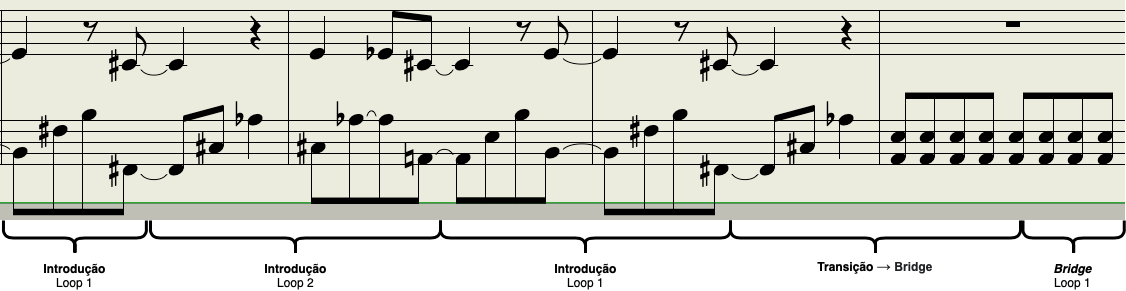
\includegraphics[width=1\textwidth]{images/dtw-window division.png}
    \caption{Relação dos estados da \figref{fig:miab_adapted_state_machine} com um corte da partitura original da trilha da guitarra elétrica da música \textit{Message In A Bottle} (\textit{The Police}, 1979). Movendo as janelas meio compasso à frente, é possível criar janelas de transição.}
    \label{fig:miab_windowed_sheet_music}
\end{figure}

Em nossos experimentos, identificamos e separamos cada estado manualmente, assim como construímos a máquina de estados de referência, semelhante à apresentada na \figref{fig:miab_adapted_state_machine}. Para a música \textit{Message In A Bottle}, utilizamos duas unidades de divisão para experimentação, uma onde cada janela de referência possuía dois compassos de duração (3,1 segundos) e outra onde possuíam um compasso de duração (1,5 segundos).

Também realizamos testes com a introdução da música \textit{Hotel California}, que, diferentemente de \textit{Message In A Bottle}, não possui \textit{loops}. Com isto, não havia necessidade da identificação de janelas de transição, tornando a máquina de estados linear. Para esta música, experimentamos durações de 2, 3 e 5 segundos para cada janela de referência.

